	
% This template from http://www.vel.co.nz, originally from http://www.tedpavlic.com

\documentclass{article}
% Change "article" to "report" to get rid of page number on title page
\usepackage{amsmath,amsfonts,amsthm,amssymb, mathrsfs}
\usepackage{bigints}
\usepackage{setspace}
\usepackage{Tabbing}
\usepackage{fancyhdr}
\usepackage{lastpage}
\usepackage{textcomp}
\usepackage{extramarks}
\usepackage{chngpage}
\usepackage{soul,color}
\usepackage{graphicx,float,wrapfig}
\usepackage{cancel}
\usepackage{indentfirst}
\usepackage{mdframed}

% In case you need to adjust margins:
\topmargin=-0.45in      %
\evensidemargin=0in     %
\oddsidemargin=0in      %
\textwidth=6.5in        %
\textheight=9.0in       %
\headsep=0.25in         %

% Homework Specific Information
\newcommand{\hmwkTitle}{WS5}
\newcommand{\hmwkDueDate}{}
\newcommand{\hmwkClass}{Ay\ 190}
\newcommand{\hmwkAuthorName}{Cutter\ Coryell}

% Setup the header and footer
\pagestyle{fancy}                                                       %
\lhead{\hmwkAuthorName}                                                 %
\chead{\hmwkClass\ : \hmwkTitle}  %
\rhead{\hmwkDueDate}                                                     %
\renewcommand\headrulewidth{0.4pt}                                      %
\renewcommand\footrulewidth{0.4pt}                                      %

% This is used to trace down (pin point) problems
% in latexing a document:
%\tracingall

%%%%%%%%%%%%%%%%%%%%%%%%%%%%%%%%%%%%%%%%%%%%%%%%%%%%%%%%%%%%%
% Some tools
\newcommand{\enterProblemHeader}[1]{\nobreak\extramarks{#1}{#1 continued on next page\ldots}\nobreak%
                                    \nobreak\extramarks{#1 (continued)}{#1 continued on next page\ldots}\nobreak}%
\newcommand{\exitProblemHeader}[1]{\nobreak\extramarks{#1 (continued)}{#1 continued on next page\ldots}\nobreak%
                                   \nobreak\extramarks{#1}{}\nobreak}%

\newlength{\labelLength}
\newcommand{\labelAnswer}[2]
  {\settowidth{\labelLength}{#1}%
   \addtolength{\labelLength}{0.25in}%
   \changetext{}{-\labelLength}{}{}{}%
   \noindent\fbox{\begin{minipage}[c]{\columnwidth}#2\end{minipage}}%
   \marginpar{\fbox{#1}}%

   % We put the blank space above in order to make sure this
   % \marginpar gets correctly placed.
   \changetext{}{+\labelLength}{}{}{}}%

\setcounter{secnumdepth}{0}
\newcommand{\homeworkProblemName}{}%
\newcounter{homeworkProblemCounter}%
\newenvironment{homeworkProblem}[1][Problem \arabic{homeworkProblemCounter}]%
  {\stepcounter{homeworkProblemCounter}%
   \renewcommand{\homeworkProblemName}{#1}%
   \section{\homeworkProblemName}%
   \enterProblemHeader{\homeworkProblemName}}%
  {\exitProblemHeader{\homeworkProblemName}}%

\newcommand{\problemAnswer}[1]
  {\noindent\fbox{\begin{minipage}[c]{\columnwidth}#1\end{minipage}}}%

\newcommand{\problemLAnswer}[1]
  {\labelAnswer{\homeworkProblemName}{#1}}

\newcommand{\homeworkSectionName}{}%
\newlength{\homeworkSectionLabelLength}{}%
\newenvironment{homeworkSection}[1]%
  {% We put this space here to make sure we're not connected to the above.
   % Otherwise the changetext can do funny things to the other margin

   \renewcommand{\homeworkSectionName}{#1}%
   \settowidth{\homeworkSectionLabelLength}{\homeworkSectionName}%
   \addtolength{\homeworkSectionLabelLength}{0.25in}%
   \changetext{}{-\homeworkSectionLabelLength}{}{}{}%
   \subsection{\homeworkSectionName}%
   \enterProblemHeader{\homeworkProblemName\ [\homeworkSectionName]}}%
  {\enterProblemHeader{\homeworkProblemName}%

   % We put the blank space above in order to make sure this margin
   % change doesn't happen too soon (otherwise \sectionAnswer's can
   % get ugly about their \marginpar placement.
   \changetext{}{+\homeworkSectionLabelLength}{}{}{}}%

\newcommand{\sectionAnswer}[1]
  {% We put this space here to make sure we're disconnected from the previous
   % passage

   \noindent\fbox{\begin{minipage}[c]{\columnwidth}#1\end{minipage}}%
   \enterProblemHeader{\homeworkProblemName}\exitProblemHeader{\homeworkProblemName}%
   \marginpar{\fbox{\homeworkSectionName}}%

   % We put the blank space above in order to make sure this
   % \marginpar gets correctly placed.
   }%

\newenvironment{myindentpar}[1]%
 {\begin{list}{}%
         {\setlength{\leftmargin}{#1}}%
         \item[]%
 }
 {\end{list}}

%%%%%%%%%%%%%%%%%%%%%%%%%%%%%%%%%%%%%%%%%%%%%%%%%%%%%%%%%%%%%


%%%%%%%%%%%%%%%%%%%%%%%%%%%%%%%%%%%%%%%%%%%%%%%%%%%%%%%%%%%%%
% Make title
\title{\vspace{2in}\textmd{\textbf{\hmwkClass:\ \hmwkTitle}}\\\normalsize\vspace{0.1in}\small{Due\ on\ \hmwkDueDate}\\\vspace{0.1in}\large{\textit{\hmwkClassInstructor\ \hmwkClassTime}}\vspace{3in}}
\date{}
\author{\textbf{\hmwkAuthorName}}
%%%%%%%%%%%%%%%%%%%%%%%%%%%%%%%%%%%%%%%%%%%%%%%%%%%%%%%%%%%%%

%%%% MY COMMANDS %%%%%%%%%%%%%%%%%%%%%

\newcommand{\deri}[2]{\frac{\mathrm{d} #1}{\mathrm{d} #2}}
\newcommand{\pderi}[2]{\frac{\partial #1}{\partial #2}}
\newcommand{\inte}[4]{\int_{#1}^{#2} \! #3 \, \mathrm{d} #4}
\newcommand{\ointe}[4]{\oint_{#1}^{#2} \! #3 \, \mathrm{d} #4}
\newcommand{\del}{\nabla}
\newcommand{\D}{\mathrm{d}}
\newcommand{\ee}[1]{\times 10^{#1}}
\newcommand{\fpe}{\frac{1}{4 \pi \epsilon_0}}
\newcommand{\bra}[1]{\left< #1 \right|}
\newcommand{\ket}[1]{\left| #1 \right>}
\newcommand{\cket}[1]{\left. #1 \right>}


% Distance units
\newcommand{\m}[0]{\text{\ m}}
\newcommand{\cm}[0]{\text{\ cm}}
\newcommand{\km}[0]{\text{\ km}}
\newcommand{\pc}[0]{\text{\ pc}}
\newcommand{\kpc}[0]{\text{\ kpc}}
\newcommand{\Mpc}[0]{\text{\ Mpc}}
\newcommand{\Gpc}[0]{\text{\ Gpc}}
\newcommand{\lyr}[0]{\text{\ lyr}}
\newcommand{\Rs}[0]{R_\odot}

% Mass units
\newcommand{\g}[0]{\text{\ g}}
\newcommand{\kg}[0]{\text{\ kg}}
\newcommand{\Ms}[0]{M_\odot}

% Time units
\newcommand{\s}[0]{\text{\ s}}
\newcommand{\days}[0]{\text{\ days}}
\newcommand{\yr}[0]{\text{\ yr}}
\newcommand{\Hz}[0]{\text{\ Hz}}
\newcommand{\kHz}[0]{\text{\ kHz}}
\newcommand{\MHz}[0]{\text{\ MHz}}
\newcommand{\GHz}[0]{\text{\ GHz}}
\newcommand{\THz}[0]{\text{\ THz}}

% Energy units
\newcommand{\erg}[0]{\text{\ erg}}
\newcommand{\J}[0]{\text{\ J}}
\newcommand{\eV}[0]{\text{\ eV}}
\newcommand{\meV}[0]{\text{\ meV}}
\newcommand{\keV}[0]{\text{\ keV}}
\newcommand{\MeV}[0]{\text{\ MeV}}
\newcommand{\GeV}[0]{\text{\ GeV}}
\newcommand{\TeV}[0]{\text{\ TeV}}

% Force units
\newcommand{\N}[0]{\text{\ N}}
\newcommand{\dyn}[0]{\text{\ dyn}}

% Power units
\newcommand{\W}[0]{\text{\ W}}
\newcommand{\Ls}[0]{L_\odot}

% Temperature units
\newcommand{\K}[0]{\text{\ K}}
\newcommand{\degC}[0]{\text{\ \(^\circ\)C}}
\newcommand{\degF}[0]{\text{\ \(^\circ\)F}}

% Electromagnetic units
\newcommand{\V}[0]{\text{\ V}}
\newcommand{\kV}[0]{\text{\ kV}}
\newcommand{\C}[0]{\text{\ C}}
\newcommand{\esu}[0]{\text{\ esu}}
\newcommand{\T}[0]{\text{\ T}}
\newcommand{\G}[0]{\text{\ G}}


\newcount\colveccount
\newcommand*\colvec[1]{
        \global\colveccount#1
        \begin{pmatrix}
        \colvecnext
}
\def\colvecnext#1{
        #1
        \global\advance\colveccount-1
        \ifnum\colveccount>0
                \\
                \expandafter\colvecnext
        \else
                \end{pmatrix}
        \fi
}

%%%%%%%%%%%%%%%%%%%%%%%%%%%%%%%%%%

\begin{document}
\begin{spacing}{1.1}

\newpage

% When problems are long, it may be desirable to put a \newpage or a
% \clearpage before each homeworkProblem environment

I worked with my Partner David Vartanyan on this worksheet. It took about three hours.

\subsection{(1) Measuring \(\pi\) with an MC Experiment}

I implemented an MC experiment that pseudo-randomly and uniformly selects points in the interval
\([0, 1] \times [0, 1]\) and determines whether or not these points are in the unit circle. By symmetry, one fourth of the unit circle is contained within this interval, so the fraction of points within the circle is an estimate of the ratio between one-fourth the circle's area (\(\frac{1}{4} \pi\)) and the area of the square interval (1). This method is demonstrated pictorially in Figure 1.

\begin{figure}[H]
\begin{centering}
 \hspace{-1cm} 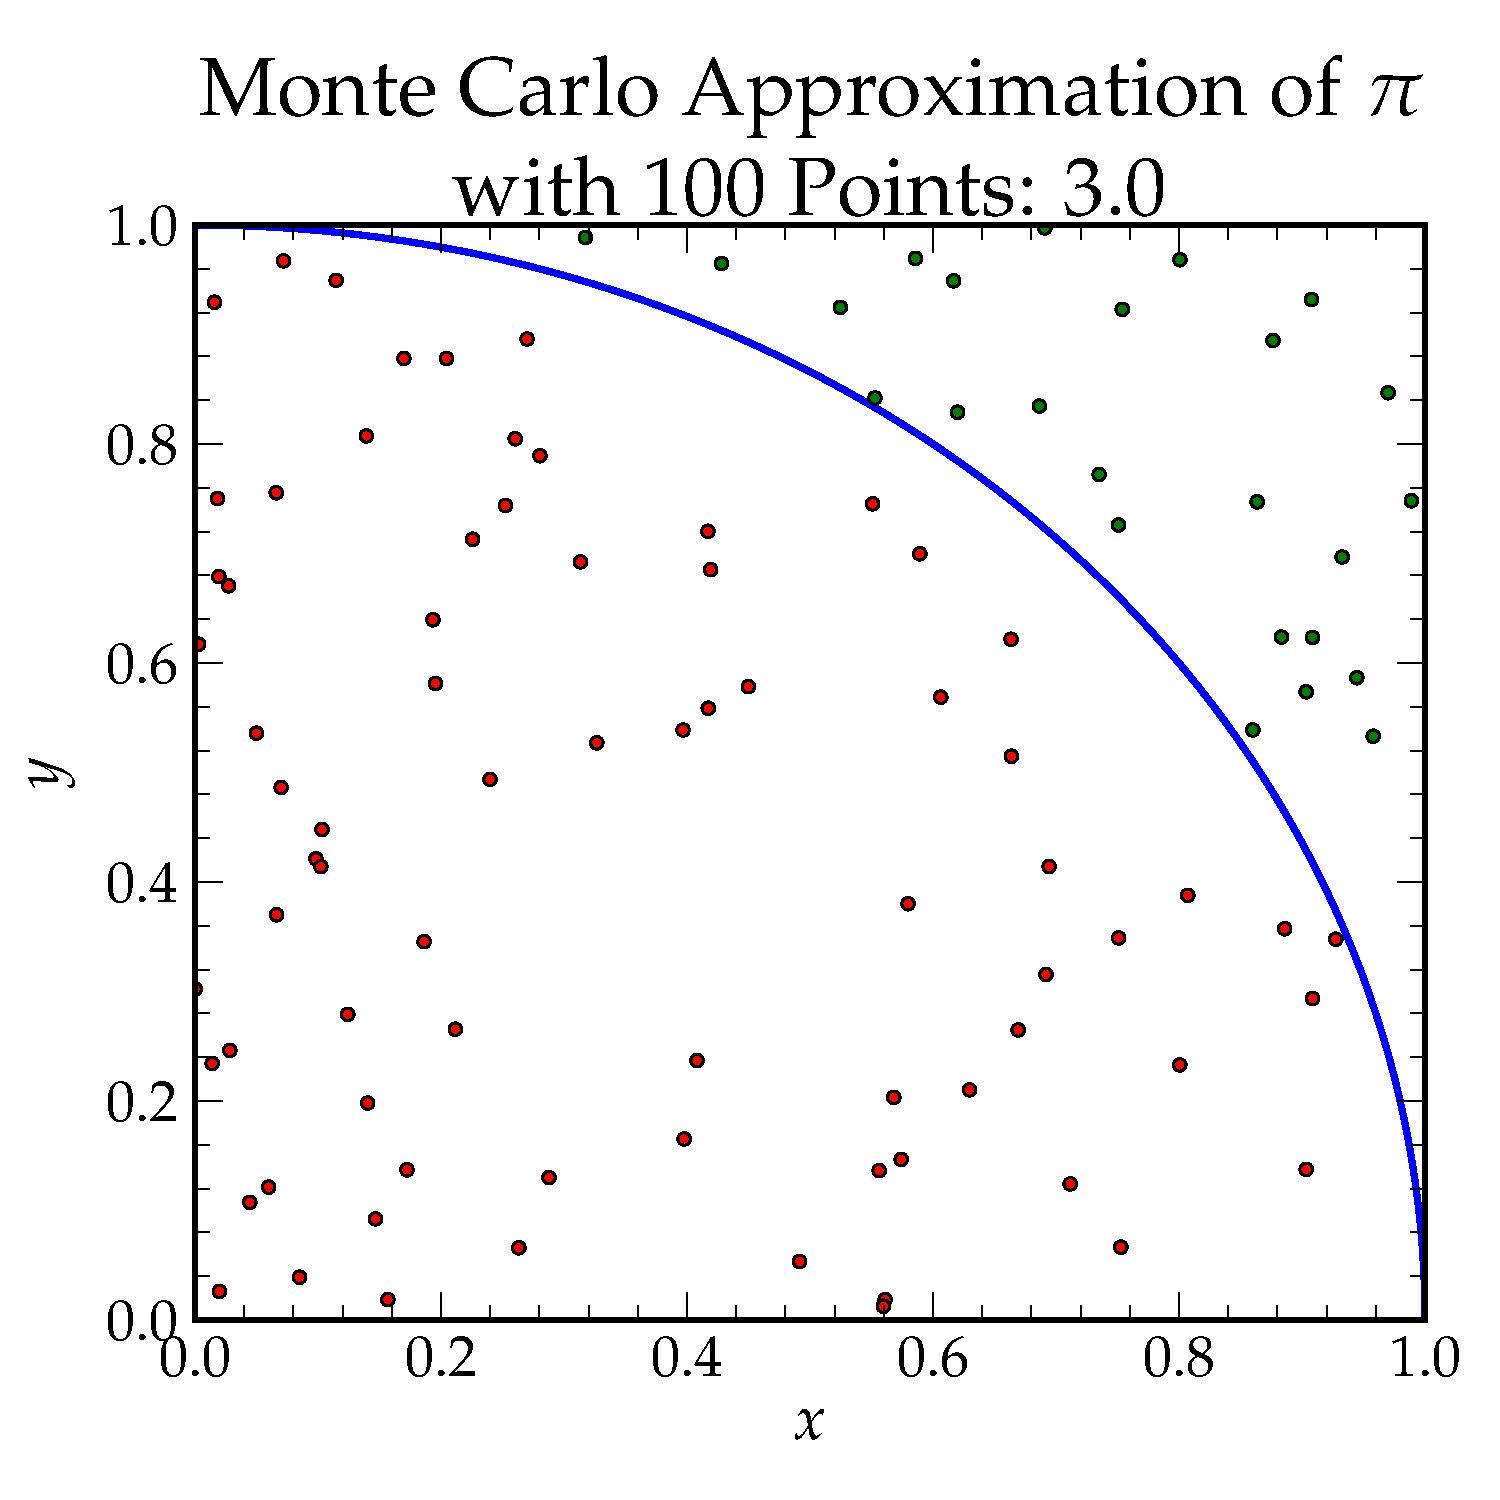
\includegraphics[width=0.8\textwidth]{fig-problem1.pdf}
 \caption{In this experiment, 75 points were internal to the circle (red) and 25 points were external (green), meaning the quarter circle has an approximate area of 0.75; the whole circle thus has approximate area 3.0.}
 \label{fig-problem1}
\end{centering}
\end{figure} 

Increasing the total number of points \(N\) by a factor of four, we should see a halving in the relative error of our scheme (since MC methods have error \(\propto N^{-1/2}\)). In the following table, we increase \(N\) in factors of four to investigate the resulting change in error.

\begin{table}[H]
\begin{centering}
\begin{tabular}{|c|c|c|}
\hline
\(N\) & Approximation of \(\pi\) & Relative Error in the Approximation \\
\hline
4 & 4.0 & 0.273 \\
16 & 3.5 & 0.114 \\
64 & 3.0 & 0.045 \\
256 & 2.984375 & 0.050 \\
1024 & 3.08984375 & 0.016 \\
4096 & 3.1474609375 & 0.002 \\
16384 & 3.13330078125 & 0.003 \\
65536 & 3.1416015625 & 0.000003 \\
262144 & 3.1450958252 & 0.001 \\
\hline
\end{tabular}
\end{centering}
\end{table}

In general at each new resolution the error goes down by a factor roughly two, but interesting at some resolutions the error seems to regress, and at some resolutions the error jumps down beyond a factor of two. I suppose that's to be expected of a probabilistic method.

\subsection{(2) The Birthday Paradox}

The result of my experiment for various numbers of trials \(N\) is given below. The analytical answer is 23, so a relative error is given.

\begin{table}[H]
\begin{centering}
\begin{tabular}{|c|c|c|}
\hline
\(N\) & Smallest Number of People & Relative Error \\
\hline
4 & 18 & 0.227 \\
16 & 23 & 0.000 \\
64 & 23 & 0.000 \\
256 & 24 & 0.045 \\
1024 & 23 & 0.000 \\
4096 & 24 & 0.045 \\
16384 & 23 & 0.000 \\
65536 & 23 & 0.000 \\
\hline
\end{tabular}
\end{centering}
\end{table}

This really doesn't appear to follow the expected convergence of \(N^{-1/2}\), but this is because we are reaching 0 error so quickly (second resolution step). There isn't really a way around this; since our trial numbers are already so small, it's hard for us to ramp up the error any more to really see the convergence behavior.

\end{spacing}
\end{document}

%%%%%%%%%%%%%%%%%%%%%%%%%%%%%%%%%%%%%%%%%%%%%%%%%%%%%%%%%%%%%
